\section{RESULT AND DISCUSSION}
\label{sec:result_and_discussion}
With the methodology used above, this project is tested in Gazebo Classic and RViz2 based on ROS2 Humble. 
The first is a reproduction of the problem to be solved in this project.
A differential robotic robot using LiDAR to build a map and avoid obstacles is formulated 
with a destination point in an indoor environment. However it accidentally collided on the way. 
Figure~\ref{fig:collision} below shows that after the collision, the constructed map becomes chaotic.
\begin{figure}[H]
    \centering
    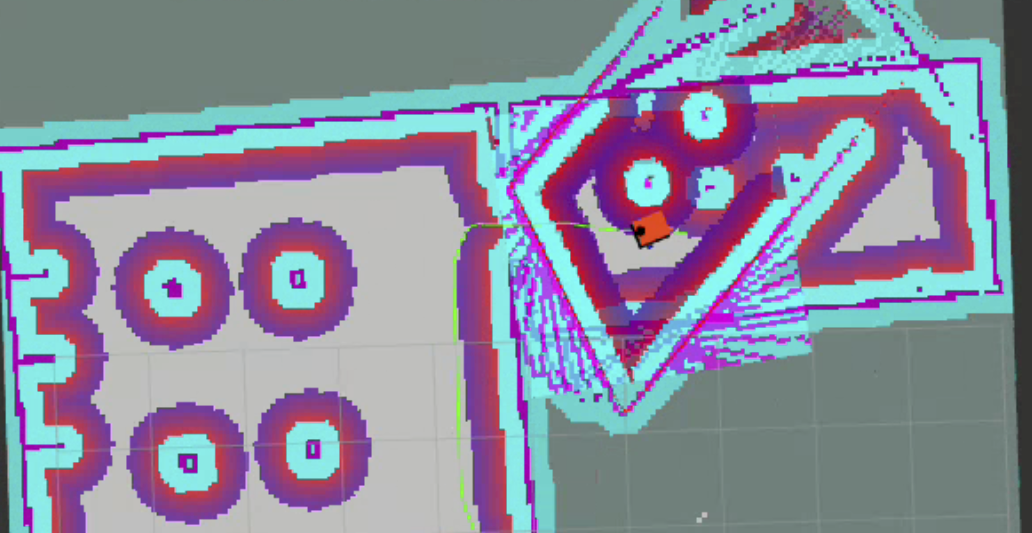
\includegraphics[width=0.4\linewidth]{figs/chaotic_map.png}
    \caption{Chaotic map after collision (top right corner)}
    \label{fig:collision}
\end{figure}
This is because the robot considers that the robot is still moving during the collision,
so the map is updated with the ``new position'' of the robot. An easy-to-understand example is the skidding that occurs in a moving car on ice. 
When the car skids, the wheels are still spinning normally, but there is no actual displacement of the car.

Two obstacles that are useful to this problem were added to the simulated world to be tested separately.
3D pointcloud mode is opened for better visualisation of the obstacles.

1. \textbf{Bookshelf}: Due to the thin partitions on each level of the bookshelf, 
the LiDAR scanning surface that is not at the same level as one of the partitions will not detect the partition, 
but only the baffles on either side. To visualise this more, the back plate of the shelf is removed 
and the shelf is then placed directly in front of the robot and mapped using only LiDAR. 
At this point it can be seen in RViz2 that only the baffles appear as obstacles in the generated map. 
If the robot is given a forward navigation command in this case, it will move straight ahead and hit the bookshelf. 
As shown in Figure~\ref{fig:bookshelf}. It will not be able to navigate correctly and at the same time it will destroy the original map.
\begin{figure}[H]
    \centering
    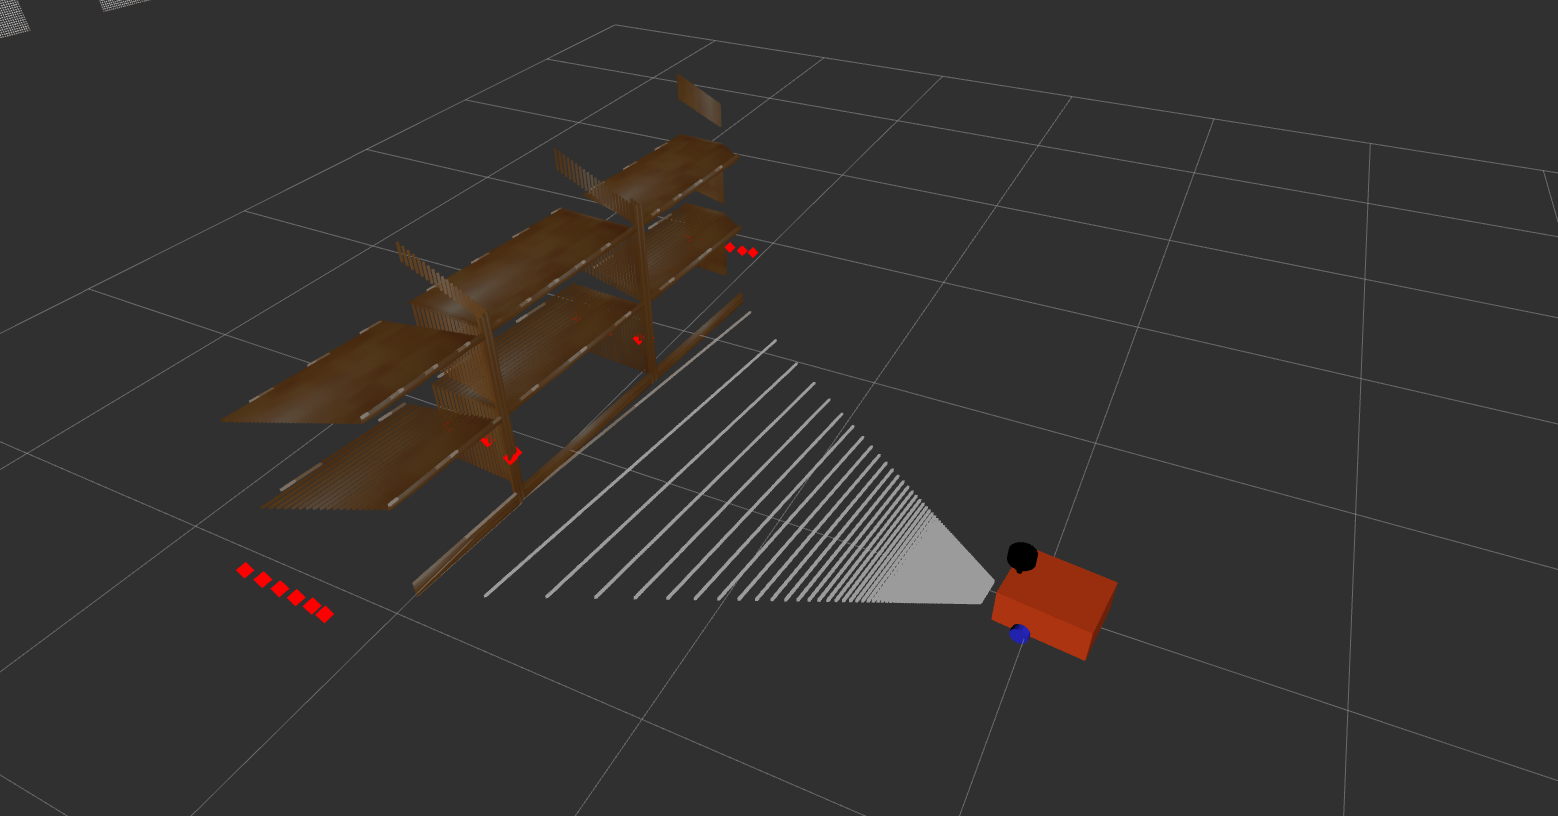
\includegraphics[width=0.8\linewidth]{figs/cannot_shelf.png}
    \caption{LiDAR cannot detect the shelf correctly}
    \label{fig:bookshelf}
\end{figure}
After using the merged LaserScan data returned by the fusion algorithm, 
it is clear in RViz2 that the baseboard of the bookshelf is successfully recognised as an obstacle and mapped.
\begin{figure}[H]
    \centering
    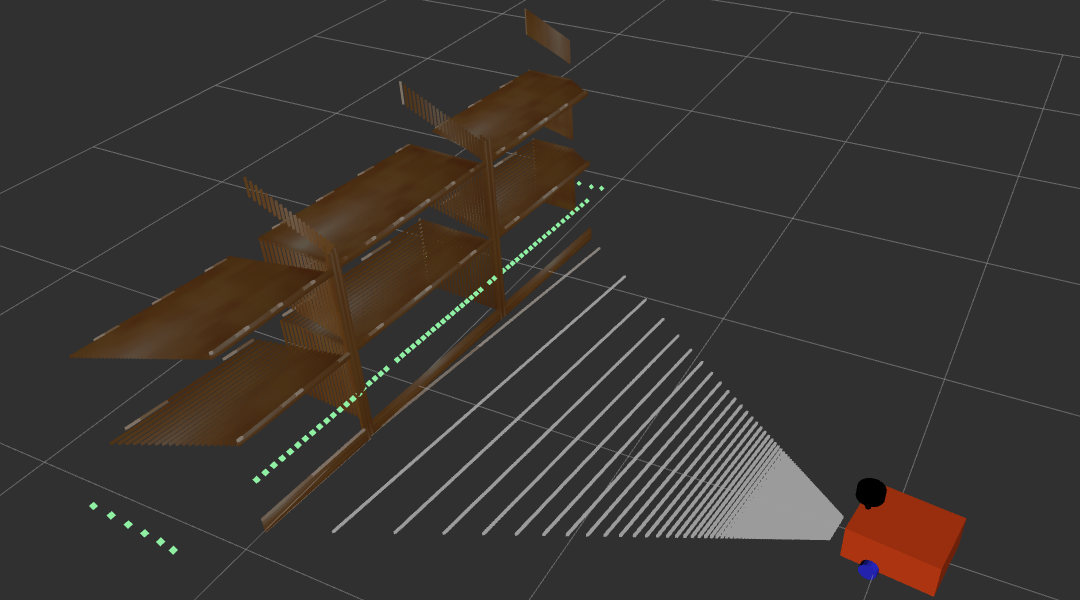
\includegraphics[width=0.8\linewidth]{figs/can_shelf.png}
    \caption{The shelf can be detected correctly after fusion}
\end{figure}
2. \textbf{Barricades}: Another very intuitive test is this cylinder barricade 
with a polygonal bottom cross-section and a rounded upper cross-section.
The different shapes of such barricades at different heights make it very straightforward 
to see whether low-lying obstacles are detected or not, 
even without the need to build a map. 
Both the LiDAR LaserScan data and the merged LaserScan data returned by the fusion algorithm, 
distinguished by different colours, are turned on in RViz2:
\begin{figure}[H]
    \centering
    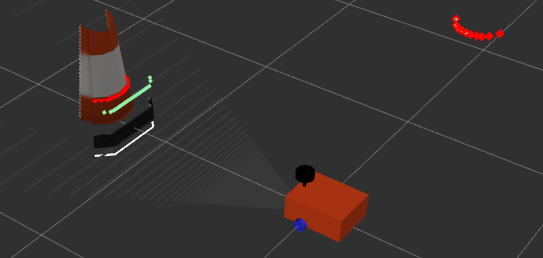
\includegraphics[width=0.8\linewidth]{figs/barricade.png}
    \caption{Different LaserScan data for same barricade}
\end{figure}
It can be seen that what is scanned before the fusion 
is the higher part of the top half with a circular cross-section.
And after the fusion, the scanning of this area is replaced with the lower part of the bottom cross-section 
with a polygonal shape. This also represents the fulfilment of the objectives of this project.




